\chapter{Общая теория внутренних гравитационных волн}
\label{cha:Theory}



\section{Математические модели для изучения внутренних гравитационных и инерционных волн}

Для описания движения несжимаемой жидкости используется уравнение Навье-Стокста. Но при небольшом перепаде плотности допустимо использовать уравнение Навье-Стокса в приближении Буссинеска, которое учитывает сжимаемость в члене с плавучестью.

\begin{equation}
 \large \frac{\partial \vec U}{\partial t} + (\vec U \cdot \nabla) \vec U = - \frac{1}{\rho_m} \nabla \hat p + \nu \Delta \vec U  + \vec f,
 \label{eq:momClassic}
\end{equation}
Уравнение переноса соли $s$:
\begin{equation}
 \large \frac{\partial \rho_s}{\partial t} + \vec U \cdot \nabla \rho_s  = \nabla \cdot \frac{\nu}{Sc} \left ( \nabla \rho_s \right ),
 \label{eq:transClassic}
\end{equation}
\begin{equation}
 \large \nabla \cdot \vec U  = 0.
 \label{eq:contClassic}
\end{equation}

Здесь $\vec{U}$ -- вестор скорости с компонентами $u_x,u_y; \nu$ -- кинематическая вязкость жидкости; $\rho_m$ -- значение плотности на верхней границе; $\rho_s$ -- добавка к плотности обусловленная наличием солености; приведенное давление $\hat{p}=p-p_0$, разница между полным и гидростатическим давлением; $\vec{f}=\frac{\rho_s}{\rho_m} \vec{g}$ -- восстанавливающая сила; Число Шмидта представляет собой отношение кинематической вязкости и коэффициента диффузии:  $Sc = \frac{\nu}{D}$. 

В данной работе помимо классических уравнений Навье-Стокса в приближении Буссинеска используются квазигидродинамические уравнения, работа над которыми ведется в институте прикладной математики имени Келдыша с восьмидесятых годов двадцатого века \cite{bookELIZ}. Различие между уравнениями Навье-Стокса несжимаемой жидкости и квазигидродинамическими уравнениями заключается в дополнительных диссипативных слагаемых. Эти слагаемые были первоначально введены для разреженного газа как способ сохранить инвариантность при пространственно-временном усреднении\cite{AIAAJ1995}. Физическая интерпретируемость в случае несжимаемой жидкости после обобщения теряется, но математически уравнения все еще верны \cite{Elizarova2011}. Как будет показано ниже диссипативные слагаемые могут быть весьма полезны при численном моделировании. 

Система приведенная ниже называется квазигидродинамической системой и впервые была получена Шеретовым \cite{ElSh2001}. Система является регуляризованным аналогом приближения Буссинеска, где $ \rho = const $.

 
Уравнение неразрывности дополняется добавочной скоростью $\vec{W}$:

    \begin{equation}
      \nabla \cdot \left (\vec U - \vec W \right ) = 0,
      \label{eq:cont}
    \end{equation}
уравнение импульса для квазигидродинамических уравнений:
\begin{equation}
      \frac{\partial \vec U}{\partial t} + \nabla \cdot \left ( (\vec U - \vec W)\otimes \vec U  \right )
      -
      \nabla \cdot \nu \left ( \nabla \vec U + (\nabla \vec U)^T \right ) - \nabla \cdot \left  (   \vec U \otimes \vec W \right )
      = 
      - \frac{1}{\rho} \nabla \Tilde{p} + \vec F,
\end{equation}
где $\nu$ - кинематическая вязкость; $\rho$ - плотность на верхней границе; $ \vec{F}$ - объемная сила; $\Tilde{p}$ давление без учета статического.

Дополнительную скорость можно записать как правую часть уравнения движения Эйлера:
\begin{equation}
      \vec W = \tau \left ( \vec U \cdot \nabla \vec U + \frac{1}{\rho} \nabla \Tilde{p} - \vec F  \right ),
      \label{eq:W}
\end{equation}

Массовая сила $\vec{F} = \beta g \Tilde{s}$ может определять поведение стратифицированной жидкости. $ \tau $ - параметр регуляризации. $ \beta $ - коэффициент соленостного сжатия $ \beta = \frac{1}{\rho}\frac{\partial \rho}{\partial s} $. В этом случае системе требуется дополнительное уравнение для отклонения начальной солености $ \Tilde{s} = s (x, y, z, t) - s (x, y, z, 0) $:

\begin{equation}
     \frac{\partial s }{\partial t} + \nabla \cdot \left ( (\vec U - \vec W) s \right )
      - \nabla \cdot \frac{\nu}{Sc} \left ( \nabla s \right ) - \nabla \cdot \left (\tau \vec{U} \cdot (\vec{U} \cdot \nabla s) \right) = 0,
\end{equation}
Уравнение для давления может быть получено напрямую путем подстановки выражения для дополнительной скорости в уравнение неразрывности \ref{eq:cont}:

\begin{equation}
     \nabla \cdot \frac{\tau}{\rho}\nabla \Tilde{p} = \nabla \cdot \left (   \vec{U} - \tau (\vec{U} \cdot \nabla \vec{U}) +  \tau \vec{F} \right ).
\end{equation}
Эти уравнение описывают движение соленой несжимаемой вязкой жидкости. Они могут быть сведены к классической системе уравнение если положить $\tau = 0$.

Для замыкания системы уравнений требуется задать граничные условия. Вход потока устанавливается как значение скорости, которое может зависеть от координат и времени по известному закону. Также необходимо определить градиент давления и солености:



\begin{equation}\label{eq:qhd_inlet}
    \vec{U} = \vec{U}_b, \,\,\, \frac{\partial \tilde p}{ \partial \vec{n}} = \rho_0 \vec n \cdot \left ( -\vec U_b \cdot \nabla \vec U + \vec F \right), \,\,\, s = s_b,
\end{equation}  

\begin{equation}\label{eq:qhd_outlet}
        \frac{\partial \vec{U}}{\partial \vec{n}} = 0, \,\,\, \tilde p = 0, \,\,\, \frac{\partial s}{ \partial \vec{n}} = 0,
\end{equation}

\begin{equation}\label{eq:qhd_walls}
        \vec{U} = 0, \,\,\, \frac{\partial \tilde p}{ \partial \vec{n}} = \rho_0 \vec n \cdot \left ( -\vec U_b \cdot \nabla \vec U + \vec F \right), \,\,\, \lambda \frac{\partial s}{ \partial \vec{n}} + \gamma s = \psi,
\end{equation}
Где $\vec U_b$ -- известное значение скорости на входе в поток,
$s_b$ -- известное значение солености на входе,
$\lambda$, $\gamma$ and $\psi$ -- специальные постоянные для переключения граничных условий между условием неймана и Дерихле скалярной величины $s$,
Граничные условия Неймана для давления определяются из следующего условия для регуляризованного потока:
$\vec n \cdot \vec W = 0$.


Таким образом описано два подхода к моделированию стратифицированной жидкости. Первый, классический представляет собой систему уравнений Навье-Стокса в приближении Буссинеска. Второй, регуляризованный представляет собой систему квазигидродинамических уравнений. 

\section{Линеаризованная теория внутренних гравитационных волн}

Ранее рассмотрена полная система уравнений, описывающая движение стратифицированной жидкости. Чтобы упростить задачу, можно предположить, что поток является двумерным и содержится в плоскости $xOz$ без изменений в направлении $y$. В этих рамках, используя уравнение неразрывности (\ref{eq:contClassic}), можно ввести функцию тока, определяемую как

\begin{equation}
    \frac{\partial \psi}{\partial x} = - u_z \;\;\;\;\;\;\;\; и \;\;\;\;\;\;\;\; \frac{\partial \psi}{\partial z} = - u_x
\end{equation}

тогда можно переписать уравнения (\ref{eq:momClassic}), (\ref{eq:transClassic}) и (\ref{eq:contClassic}) как

\begin{equation}
    \partial_{tz} \psi + J(\partial_z \psi, \psi) = - \frac{1}{\rho} \partial_x P + \nu \partial_z \Delta \psi,
    \label{eq:tokz}
\end{equation}

\begin{equation}
    \partial_{tx} \psi + J(\partial_x \psi, \psi) = \frac{\rho_s}{\rho_m}\vec{g}+\frac{1}{\rho}\partial_z P + \nu \partial_x \Delta \psi,
    \label{eq:tokx}
\end{equation}

\begin{equation}
    \partial_t \rho_s + J(\rho_s,\psi) = \nabla \cdot \frac{\nu}{Sc} (\nabla \rho_s) + \frac{d \rho}{dz} \partial_x \psi,
\end{equation}
где $J$ это яклбиан определенный как $J(f,g) = \partial_x f \partial_z g - \partial_z f \partial_x g.$ Обозначим как $\partial_j \psi =\frac{\partial \psi}{\partial j}$, где $j$ обозначает $x,y$ или $t$. 

В дальнейшем предполагается, что возмущения плотности $\rho_s(x; z; t)$ малы по сравнению с фоновой стратификацией $\rho(z)$. Это предположение полностью верно как в океане, так и экспериментах, рассматриваемых тут. Таким образом, возмущения плотности ограничиваются менее чем 10\% средней стратификации. 

Дифференцируя уравнение (\ref{eq:tokz}) по $z$, а (\ref{eq:tokx}) по $x$ и складывая их получаем

\begin{equation}
    \partial_t(\Delta \psi) + J (\Delta \psi, \psi) - \nu \Delta (\Delta \psi) = \frac{g}{\rho_m} \partial_x \rho_s,
    \label{eq:tokzz}
\end{equation}

\begin{equation}
    \partial_t \rho_s + J(\rho_s,\psi) - \nabla \cdot \frac{\nu}{Sc} (\nabla \rho_s) = -N^2 \frac{\rho_m}{g}\partial_x \psi.
    \label{eq:tokxx}
\end{equation}

Уравнения (\ref{eq:tokzz}) и (\ref{eq:tokxx}) описывают нелинейную динамику вязкой стратифицированной жидкости с диффузией. Уравнения для линейной динамики получаются путем пренебрежения нелинейными членами. Это приводит к

\begin{equation}
    \partial_t(\Delta \psi) + \nu \Delta (\Delta \psi) = \frac{g}{\rho_m} \partial_x \rho_s,
\end{equation}

\begin{equation}
    \partial_t \rho_s - \nabla \cdot \frac{\nu}{Sc} (\nabla \rho_s) = -N^2 \frac{\rho_m}{g}\partial_x \psi.
\end{equation}

Рассмотрим решение в виде плоской волны к линеаризованной системе: $\psi = \psi_0 exp(i\omega t - i \vec{k} \cdot \vec{r})$ и $\rho_s=\rho_m exp(i\omega t - i \vec{k}\cdot \vec{r})$. Волновой вектор $\vec{k}=k_x \vec{e}_x + k_z \vec{e}_z$ и его модуль $k$.

Линейная система может быть записана в матричном виде

\begin{equation}
    \left(\begin{array}{cc} -k^2(i\omega + \nu k^2) & i \frac{g}{\rho_m}k_x
    \\[15pt] iN^2 \frac{\rho_m}{g}kx & i\omega + \frac{\nu}{Sc} k^2 \end{array}\right)
    \left(\begin{array}{c}\psi \\[15pt] \rho_s\end{array}\right) = 
    \left(\begin{array}{c}0 \\[15pt] 0\end{array}\right).
\end{equation}

Можно найти нетривиальное решение этой системы

\begin{equation}
    k^2 \left( i\omega + \nu k^2 \right) \left(i \omega \frac{\nu}{Sc} k^2 \right) + N^2 k^2_x = 0.
\end{equation}

Если рассмотреть систему без диссипативных членов, убрать диффузию и теплопроводность то уравнение примет вид:

\begin{equation}
    \left(\frac{\omega}{N}\right)=\frac{k^2_x}{k^2} \;\;\;\;\;\;\;\; или \;\;\;\;\;\;\;\; \frac{\omega}{N}=\pm \frac{|k_x|}{k}.
\end{equation}

Это дисперсионное соотношение линейных внутренних волн в невязкой и недиффузионной жидкости. Его можно записать, используя угол $\theta$ между вертикальной осью $z$ и волновым вектором $\vec{k}$

\begin{equation}
    \frac{\omega}{N} = \pm sin \theta.
    \label{eq:dispersion}
\end{equation}

Это чисто геометрическое соотношение, которое показывает как распространяются волны в стратифицированной жидкости(Рис. \ref{fig:ermExp}). Угол распространения определяется только частотой плавучести и частотой вынужденных колебаний. Наконец, стоит отметить, что в дисперсионном соотношении отсутствует характерный масштаб длины. Таким образом, длина внутренних волн определяется граничными условиями, только источником волн.

\begin{figure}
    \centering
    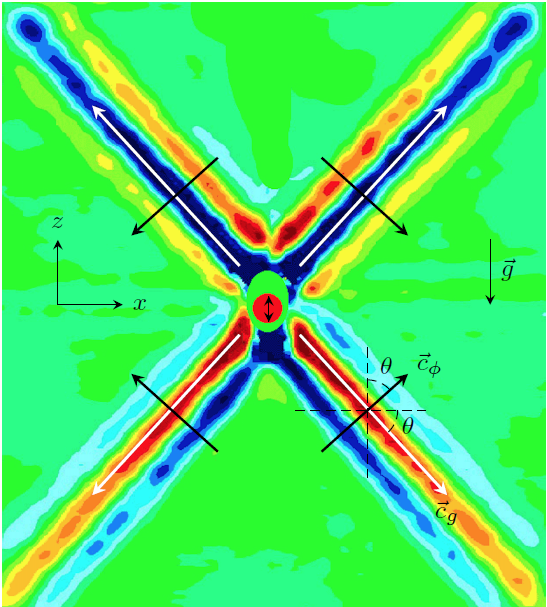
\includegraphics[scale=0.5]{Figs/Experement_Erm.png}
    \caption{Внутренние волны, излучаемые вертикально колеблющимся цилиндром, распространяются в линейно стратифицированной жидкости и  показаны красным в центре рисунка. Векторы групповой скорости показаны белым цветом, а векторы фазовой скорости - черным. Цветами обозначены поля горизонтального градиента плотности, полученные экспериментально Евгением Ерманюком с использованием методики SyS. Рисунок из \cite{brouzet:tel-01361201}}
    \label{fig:ermExp}
\end{figure}

%\subsection{Численные методы исследования волновых течений в неоднородных средах}


\section{Исследование свойств волновых течений с помощью трассировки лучей}

Дисперсионное соотношение дает мощный инструмент позволяющий качественно предсказать траекторию движения пучков внутренних волн, не только по удалению от источника но и при отражении от припятский(Рис. \ref{fig:internalReflection}). Поле отражения внутренняя волна сохраняет угол с вертикалью. Кроме того внутренние волны обладают ствойством фокусировки что выражается в сокращении расстояния между двумя параллельно пущенными лучами поле отражения от наклонной стенки. 

\begin{figure}
    \centering
    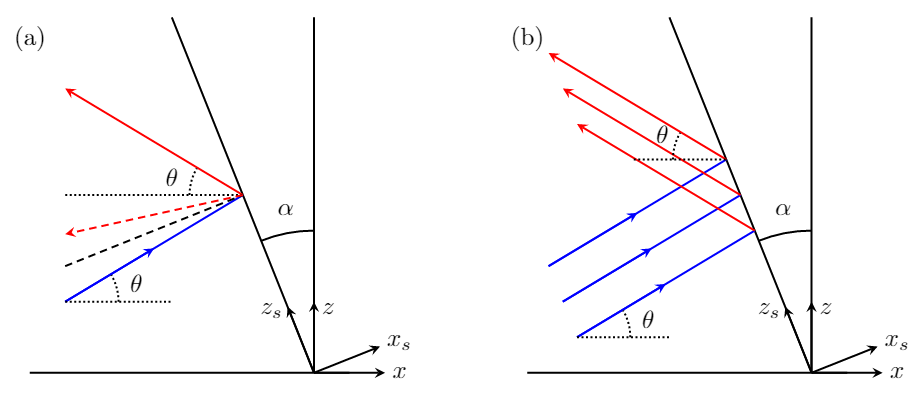
\includegraphics[scale=0.5]{Figs/angle_of_reflection.png}
    \caption{Отражение пучка внутренних волн от наклонной стенки. а) Отражение одного пучка, падающий волновой луч изображен синим цветом, отраженный от наклонной стенки красным, точками обозначена биссектрисса. Черным пунктиром обозначен перпендикуляр к наклонной поверхности, красным пунктиром луч отраженный <<зеркально>> по правилу Евклида. b) Отражение нескольких волновых лучшей от наклонной поверхности, отраженные лучи стали ближе, чем были падающие.}
    \label{fig:internalReflection}
\end{figure}

Трассировка лучей позволяет последовательно проследовать по траектории движения линейных внутренних волн без дисперсии и диффузии. В 1995 году Лео Маас обнаружил, что в трапециевидном резервуаре после множественных отражений внутренние волны зацикливаются около траектории которая имеет форму параллелограмма\cite{Maas1995}. Рис. \ref{fig:RayTr} показывает результат трассировки лучей в трапециевидном резервуаре.

\begin{figure}
    \centering
    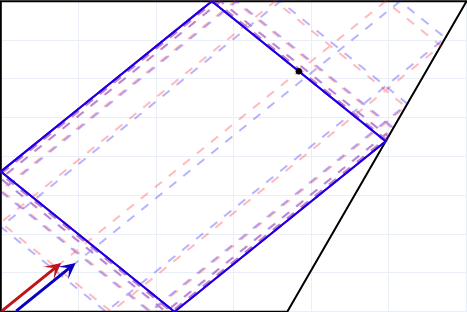
\includegraphics[scale=0.8]{Figs/RayTracing.png}
    \caption{Результат многократного отражения двух параллельных лучей внутренних волн}
    \label{fig:RayTr}
\end{figure}

Говоря о трассировки лучей нельзя не упомянуть о диаграмме Мааса\cite{Maas1997}. В задачах моделирования аттрактора имеется множество параметров:

\begin{itemize}
    \item Угол наклона стенки
    \item Частота плавучести
    \item Частота колебаний волнопродуктора
    \item Длинна резервуара
    \item Высота резервуара
\end{itemize}

Задачу трассировки лучей можно упростить, введя параметры. В своей работе он предлагает параметризовать резервуар фокусировки внутренних волн следующим образом(Рис. \ref{fig:domainTran}):

Применяется преобразование горизонтальной координаты, которое перемещает систему координат таким образом чтобы левый конец резервуара соответствовал координате $-1$ а правый $1$. Вводится параметр $d$ который обозначает расстояние от нуля новой горизонтальной оси до точки соприкосновения наклонной стенки с горизонтальной осью.
\begin{equation}
    x'=\frac{x\cdot 2}{L_1}-1
    \label{eq:transformX}
\end{equation}

Затем преобразование вертикальной координаты, которое сжимает или растягивает высоту резервуара так чтобы угол отражжения и распространения внутренних волн стал $45^\circ$. При этом вводится параметр $\tau$, который обозначает новую высоту резервуара. 
\begin{equation}
    z'=\frac{z\cdot 2}{L_1}\sqrt{\frac{N^2}{\omega^2}-1}
    \label{eq:transformZ}
\end{equation}

Таким образом вместо пяти определяющих параметров для геометрической задачи, остаются всего два, $d$ и $\tau$.

Благодаря методу трассировки лучей можно геометрически предсказать форму аттрактора внутренних волн. 

\begin{figure}
    \begin{subfigure}{\textwidth}
    \centering
    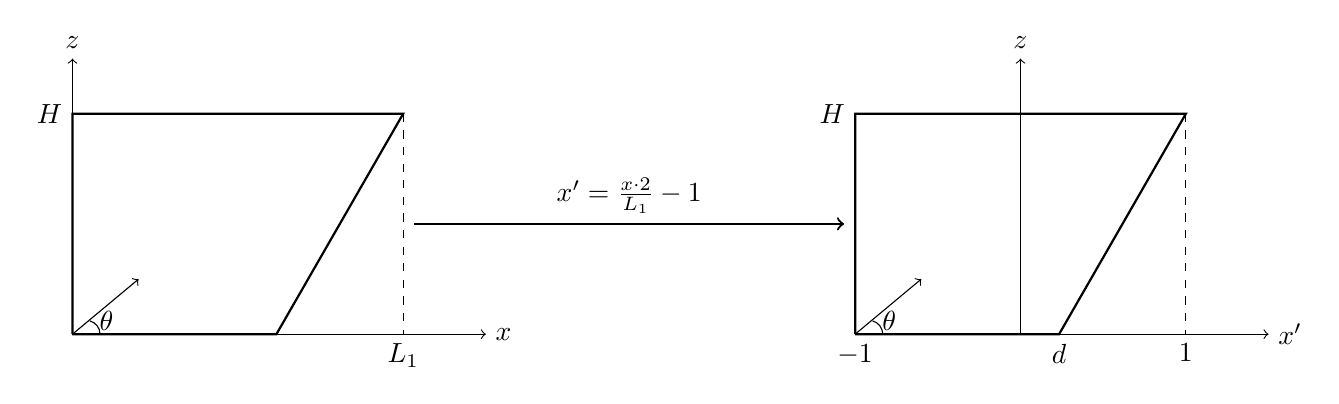
\begin{tikzpicture}[scale=0.7]
        \draw[thick] (0,0)--(0,4)node[left]{$H$}--(6,4)--(3.7,0)--(0,0);
        \draw[dashed] (6,4) -- (6,0)node[below]{$L_1$};
        \draw[thick,->] (6.2,2)->node[above]{$x'=\frac{x\cdot 2}{L_1}-1$}(14,2);
        \draw[->] (0,0)->(0,5)node[above]{$z$};
        \draw[->] (0,0)->(7.5,0)node[right]{$x$};
        \draw[->] (0,0)->(1.2,1);
        \draw[black] (0.5,0) arc [start angle=0, end angle=75, radius=0.25cm] node [right] {$\theta$};
        \draw[thick] (14.2,0)node[below]{$-1$}--(14.2,4)node[left]{$H$}--(20.2,4)--(17.9,0)node[below]{$d$}--(14.2,0);
        \draw[dashed] (20.2,4) -- (20.2,0)node[below]{$1$};
        \draw[->] (17.2,0)->(21.7,0)node[right]{$x'$};
        \draw[->] (17.2,0)->(17.2,5)node[above]{$z$};
        \draw[->] (14.2,0)->(15.4,1);
        \draw [black] (14.7,0) arc [start angle=0, end angle=75, radius=0.25cm] node [right] {$\theta$};
    \end{tikzpicture}
    \caption{Горизонтальное преобразование расчетной области}
    \end{subfigure}
    
    \begin{subfigure}{\textwidth}
    \centering
    \begin{tikzpicture}[scale=0.7]
        \draw[thick] (0,0)--(0,4)node[left]{$H$}--(6,4)--(3.7,0)--(0,0);
        \draw[dashed] (6,4) -- (6,0)node[below]{$L_1$};
        \draw[thick,->] (6.2,2)->node[above]{$z'=\frac{z\cdot 2}{L_1}\sqrt{\frac{N^2}{\omega^2}-1}$}(14,2);
        \draw[->] (0,0)->(0,5)node[above]{$z$};
        \draw[->] (0,0)->(7.5,0)node[right]{$x$};
        \draw[thick] (14.2,0)--(14.2,4.8)node[left]{$\tau$}--(20.2,4.8)--(17.9,0)--(14.2,0);
        \draw[black] (0.5,0) arc [start angle=0, end angle=75, radius=0.25cm] node [right] {$\theta$};
        \draw [black] (14.7,0) arc [start angle=0, end angle=80, radius=0.25cm] node [right] {$45^\circ$};
        \draw[->] (0,0)->(1.2,1);
        \draw[->] (14.2,0)->(15.4,1.2);
        \draw[dashed] (20.2,4.8) -- (20.2,0)node[below]{$L_1$};
        \draw[->] (17.2,0)->(21.7,0)node[right]{$x$};
        \draw[->] (14.2,0)->(14.2,6)node[above]{$z'$};
    \end{tikzpicture}
    \caption{Вертикальное преобразоввание расчетной области}
    \end{subfigure}
    \caption{Преобразования расчетной области для процедуры получения диаграммы Мааса}
    \label{fig:domainTran}
\end{figure}

На рисунке 

\begin{figure}
    \begin{subfigure}[с]{0.45\textwidth}
        \centering
        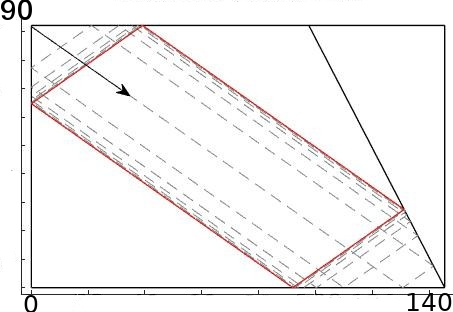
\includegraphics[scale=0.45]{Figs/RayTr923x1455.jpeg}
        \caption{Трассировка лучей,\\ $H=92.3$, $L=145.5$, $\theta = 35.13^{\circ}$,\\ $\alpha = 27.4^{\circ}$}
    \end{subfigure}
    \begin{subfigure}[r]{0.45\textwidth}
        \centering
        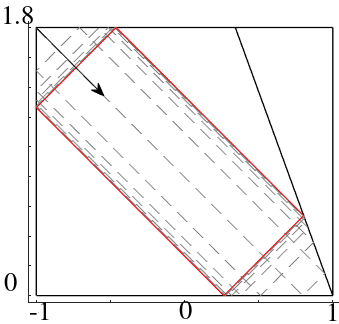
\includegraphics[scale=0.45]{Figs/RTdtau.png}
        \caption{Трассировка лучей в преобразованной геометрии, \\ $\tau = 1.8$, $d = 0.34$}
    \end{subfigure}
    
    
    \caption{Результат работы процедуры трассировки лучей и результат перехода к универсальным координатам $(d,\tau)$}


    \label{fig:RayTr923x1455}
\end{figure}
